\section*{Figure captions:}
\begin{figure}[H]
\begin{center}
\scalebox{0.75}{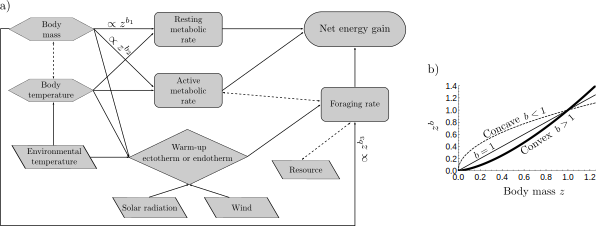
\includegraphics{fig1}}
\caption{
	A caricature of how the exponent influences the concavity (convexity)of the power law relationship.
	The black and gray lines represent foraging (gain) and  metabolic rates (cost).
	The coefficient of the metabolic rate is a bit lower to visualize cases where that the gain is more than the cost.
}
\label{fig1}
\end{center}
\end{figure}
%\vspace{-1.5cm}
%\newpage
%
\begin{figure}[H]
\begin{center}
\scalebox{0.90}{\includegraphics{fig2}}
\caption{
	No warm-up and resource is limiting.
	Daily net energy gain  $E_n$ as function body mass $z$ for different value of foraging exponent $b_3 = 0.5, 0.8, 1.25$, dashed, thin, thick lines respectively.
	The upper panels depict different resource availabilities at $15 ^{\circ} \rm{C}$. 
	Low resource = 2.5, intermediate resource= 20, unlimited resource means an individual can collect 50 times its body mass, $b_2 = 0.75, a_2 = 20 a_1$. 
	The lower panels depict the influence of temperature when resources are unlimited and high active metabolic rate $a_2 = 40 a_1, b_2  = 1.25$.
	Low, mild, and high temperature = $5, 15, 25^{\circ} \rm{C}$.
	Fixed parameter values: $b_1 = 0.75, \rho = 16$.
}
\label{fig2}
\end{center}
\end{figure}
%\vspace{-1.5cm}
\newpage
%
\begin{figure}[H]
\begin{center}
\scalebox{0.85}{\includegraphics{fig3}}
\caption{
	No warm-up and foraging time is limited to 0.5 hour.
	a) Daily net energy gain  $E_n$ as function body mass $z$ for different value of foraging exponent $b_3 = 0.5, 0.8, 1.25$, dashed, thin, thick lines respectively  at $15 ^{\circ} \rm{C}$.
	b) $E_n$ is maximized at intermediate value of $z$  when shaded regions and resource quality $\rho$ intersect (i.e., \cref{C1} is satisfied).
	Warm ($35^{\circ} \rm{C}$) and cold (15$^{\circ} \rm{C}$) environmental temperatures are denoted by red and cyan, respectively.
	The upper (lower) limit of the shade region is $\widetilde{dE_n}$ ($\widetilde{E_n}$).  
	c) Various shapes of $E_n$ based on b).
	In b) and c), $\rho = 13, 60, 100$ dashed, thin, and thick, respectively.
	Fixed parameter values: $b_1 = b_2 = 0.75, a_2 = 5 a_1, $.
}
\label{fig3}
\end{center}
\end{figure}
%\vspace{-1.5cm}
%\newpage
%
\begin{figure}[H]
\begin{center}
\scalebox{0.85}{
\includegraphics{fig4}}
\caption{
	Lowest temperature required for the completion of warm-up as a function of body mass.
	The individual is given a maximum of 6 hours to complete warm-up.
	The thorax is half of the total body mass.
	To focus on the effect of solar radiation, daily temperature is constant.
	Solar radiation increases linearly from 0 to 0.25 of the maximum value $S_0$ during a period of 6 hours. 
	a) conductance is low (0.1 $\times$ the default value).
	b) conductance is default, wind speed  = 0.1m/s.
	c) For endotherm with free convection $a_w = 1.25$. 
	Fixed parameter values: default conductance $K_1 = 0.05 c_p, r_3 = 0.5$.
	Remaining parameters are in table 1.
}% Add parameter values later
\label{fig4}
\end{center}
\end{figure}
%\vspace{-1.5cm}
%\newpage
%
\begin{figure}[H]
\begin{center}
\scalebox{0.85}{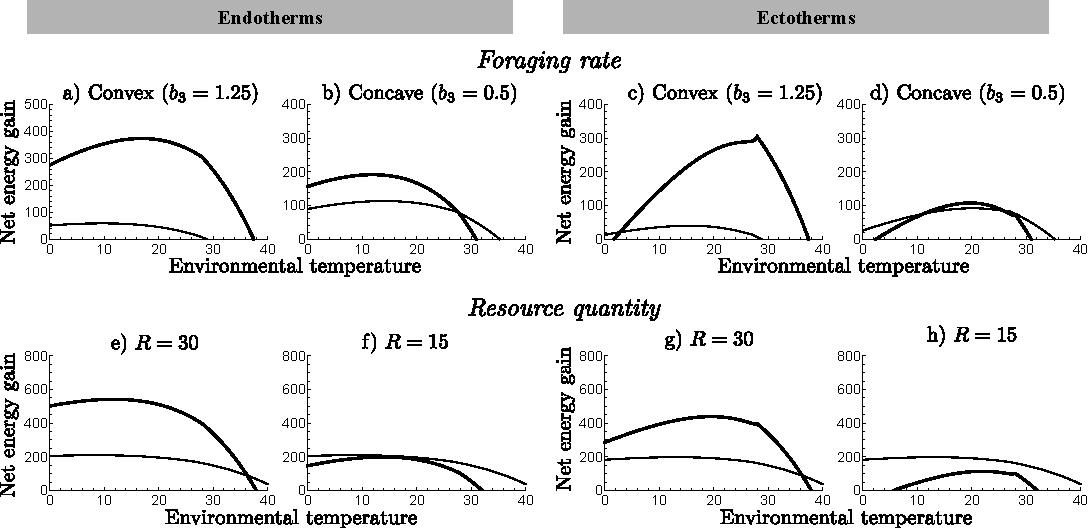
\includegraphics{fig5}}
\caption{
	Duration of warm-up as a function of the timing of warm-up.
	Daily temperature varies from $15^{\circ}\rm{C}$ at sunrise and peaks at $30^{\circ}\rm{C}$ in the middle of the afternoon.
	Solar radiation is equivalent to what would happen at 30 degree latitude during to equinox clear sky.
	a) thickest, thick, thin, and dashed lines denote  $z = 10, 1, 0.01$,  respectively.
	b)  Duration of warm-up with different conductance. Body size $z = 1$ , $a_w = 1.25$
	Default value for $K_1$ and $K_2$ .	
}% Add parameter values later
\label{fig5}
\end{center}
\end{figure}
\vspace{-0.85 cm}
%\newpage
%%
\begin{figure}[H]
\begin{center}
\scalebox{0.80}{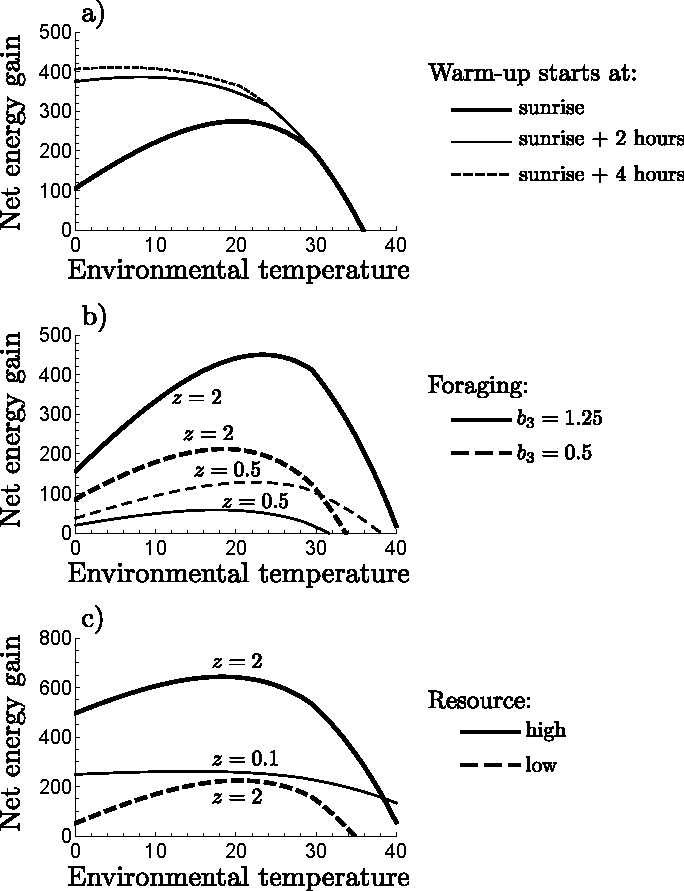
\includegraphics{fig6}}
\caption{
	Shape of the fundamental niche as a function of temperature.
	a) As a function of when warm-up starts ($\tau_f = 1$ hour and body size $z = 2$). %, early = sunrise, mid = sunrise+ 2 hr, late = sunrise + 4 hr 
	b) As a function of the exponent of $b_3$ ($\tau_f = 1$, large (black) = 2, small (gray) = 0.5).
	c)  As a function of resource availability. 
	Thick line = high resource (30), thin line = low resource (15).
	Thick and thin gray lines overlap because the small is not affected by resource loss. 
	  ($b_3 = b_2 = b_1 = 0.75$).
	Other parameters: $ b_2 = b_1  = 0.75,  a_2 = 10 a_1, a_w = 1.25$, and  $\rho = 30$.
}% Add non trivial units later
\label{fig6}
\end{center}
\end{figure}
%
%\begin{figure}[H]
%\begin{center}
%%\scalebox{1.5}{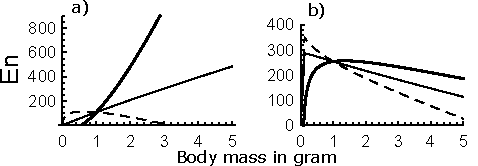
\includegraphics{Fig1}}
%\caption{
%	Shape of the fundamental niche as a function of temperature.
%	Except in d),  temperature is constant during the day.
%	a) The simplest case without warm-up, high resource availability (30 gram).
%	b) Halving resource availability and without warm-up.
%	c) Adding warm-up and  restoring resource availability to high, there is a penalty for long warm-up time as it reduces total foraging time, no change in temperature.
%	d) A complete  scenario with warm-up and variable temperature that increases from 15 to $30^{\circ} \rm{C}$ from sunrise to mid-afternoon.
%	Other parameters: $b_3 = 1, b_2 = b_1  = 0.75,  a_2 = 10 a_1, a_w = 1.25$, and  $\rho = 20$.
%}% Add non trivial units later
%\label{fig6}
%\end{center}
%\end{figure}
%